\chapter{Elements of a project}

A project in \textbf{\texttt{co2amp}} must include the following elements, each specified in separate input YAML ('.yml') files:
\begin{enumerate}
    \item One or more \texttt{pulses}
    \item One or more \texttt{optics}
    \item One \texttt{layout}
\end{enumerate}
Each element is detailed in its dedicated YAML file\footnote{\textbf{\texttt{co2amp}} additionally requires an input file 'config\_files.yml' that enumerates all input YAML files and the types of corresponding elements. \textbf{\texttt{co2amp+}} automatically generates this file.}. The last \texttt{optic} in the \texttt{layout} must be of type P (\textit{Probe}).

The subsequent sections provide brief descriptions of each of these elements and the models associated with them. For a comprehensive understanding, refer to the templates, example files, and the comments within them.


%%%%%%%%%%%%%%%%%%%%%%%%%%%%%%%%%%%%%%%%%%%%%%%%%%%%%%%%%%%%%%%%%%%%%%%%%%%%%%%%%
\section{\texttt{Pulse}}
Unless utilizing the output of another project (a '.pulse' file) as input, both the temporal and spatial shape of the input \texttt{pulse} must be defined in a corresponding YAML ('.yml') file. The \texttt{pulse} is assumed to be transform-limited, meaning it has no initial chirping. Specifications such as the \texttt{pulse} energy, central frequency, and injection time are also required. The injection time denotes the time-delay between the zero moment of the laboratory time frame ("slow" time frame) and the injection of a \texttt{pulse} into the optical system (the first \texttt{optic} in the \texttt{layout}). An example of a \texttt{pulse} configuration file is provided below.

\begin{verbatim}
#=========================
# PULSE.yml from 'examples/00 simple propagation.co2' project

t_in: 0
E: 1e-3
freq: 32.5e12

beam: GAUSS
w: 3e-3

pulse: GAUSS
fwhm: 2e-12
#=========================
\end{verbatim}

This file specifies a 2~ps (FWHM) transform-limited Gaussian pulse with a $w=3$~mm Gaussian beam profile, 1~mJ energy, and a 32.5~THz central frequency, injected into the system at $t_{\text{in}}=0$. Several pre-defined beam and pulse profile options are available, such as \texttt{GAUSS}, \texttt{FLATTOP}, \texttt{SUPERGAUSS4}, \texttt{SUPERGAUSS6}, etc. Alternatively, a \texttt{FREEFORM} option allows for the specification of an arbitrary shape through a tabulated numerical profile (refer to the 'pulse.yml' template for details).


%%%%%%%%%%%%%%%%%%%%%%%%%%%%%%%%%%%%%%%%%%%%%%%%%%%%%%%%%%%%%%%%%%%%%%%%%%%%%%%%%
\section{\texttt{Layout}}
\subsection{Configuration}
The \texttt{layout} configuration defines the sequence of \texttt{optics} and the distances between them in the optical system. Below is an example of a simple \texttt{layout} configuration file:

\begin{verbatim}
#=========================
# LAYOUT.yml from 'examples/00 simple propagation.co2' project

- go: P1 >> 3 >> P2
  times: 1
#=========================
\end{verbatim}

In this example, the system consists of two \texttt{optics}, \texttt{P1} and \texttt{P2}, separated by 3 meters of free space. The pulses pass through the system once. If the \texttt{times} value is greater than 1, a pulse after passing through \texttt{P2} will return to \texttt{P1}, and the propagation through the system will repeat for the specified number of times. A \texttt{layout} configuration file can contain several such "go-times" sequences. Below is an example of a \texttt{layout} configuration for a more complex system:

\begin{spverbatim}
#=========================
# LAYOUT.yml from 'examples/ATF 5 TW/ATF 1 regen.co2' project

- go: str >> COU1
  times: 1

- go: 0.45 >> i >> 0.90 >> GE >> 0.25 >> w >> WIN1 >> w >> 0.45 >> AM1 >> 0.40 >> AM2 >> 0.45 >> w >> WIN2 >> w >> 0.10 >> MIR >> m >> 0.10 >> w >> WIN2 >> w >> 0.45 >> AM2 >> 0.40 >> AM1 >> 0.45 >> w >> WIN1 >> w >> 0.25 >> GE >> 0.90 >> i >> 0.45 >> COU2
  times: 15

- go: 0.45 >> i >> 0.90 >> GE >> 0.25 >> w >> WIN1 >> w >> 0.45 >> AM1 >> 0.40 >> AM2 >> 0.45 >> w >> WIN2 >> w >> 0.10 >> MIR >> m >> 0.10 >> w >> WIN2 >> w >> 0.45 >> AM2 >> 0.40 >> AM1 >> 0.45 >> w >> WIN1 >> w >> 0.25 >> OUT
  times: 1
#=========================
\end{spverbatim}


\subsection{Dealing with Long Optical Elements}
In the \textbf{\texttt{co2amp}} model, \texttt{optics} are considered infinitely thin. For long \texttt{optics}, such as an \textit{Active Medium}, the model calculates the field modification accumulated by a \texttt{pulse} as it propagates through the \texttt{optic} and then applies this modification as if it occurred instantaneously. However, this approach might not be accurate if the actual optical element is lengthy and the \texttt{pulse} changes significantly while propagating through it, thereby interacting differently with various parts of the \texttt{optic}. The model's accuracy can be improved by dividing long elements into shorter sub-sections.

Fig.~\ref{fig:layout} illustrates an example of a 2-meter long \texttt{layout} with a meter-long active medium in the middle. In one scenario, shown in Fig.~\ref{fig:layout}a, we first propagate the \texttt{pulse} to the midpoint of the amplifier section, then apply the amplification accumulated over 1 meter, and finally propagate the \texttt{pulse} to the last \texttt{optic}.
\begin{figure}[ht]
\centering
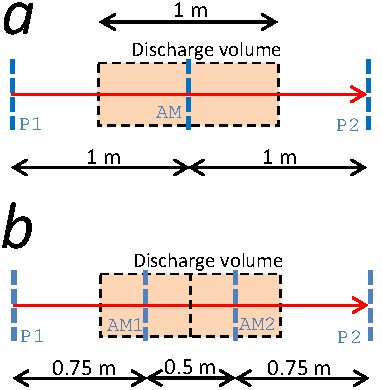
\includegraphics{images/layout}
\caption{Example of \texttt{layout} configuration for a long \texttt{optic} (in this case, an \textit{Active Medium}). a) The \textit{Active Medium} is represented by a single \texttt{optic}. b) The \textit{Active Medium} is split into two shorter sections.}\label{fig:layout}
\end{figure}
The corresponding \texttt{layout} configuration is:

\begin{verbatim}
#=========================
# long amplifier

- go: P1 >> 1 >> AM >> 1 >> P2
  times: 1
#=========================
\end{verbatim}

Alternatively, the active medium can be represented by two 0.5-meter sections, as shown in Fig.~\ref{fig:layout}b. The corresponding layout is:

\begin{verbatim}
#=========================
# long amplifier divided into two shorter sections

- go: P1 >> 0.75 >> AM1 >> 0.5 >> AM2 >> 0.75 >> P2
  times: 1
#=========================
\end{verbatim}

By splitting a long amplifier into shorter sections, the population dynamics within each amplifier section is modeled more accurately, leading to a more realistic representation of the active medium.


%%%%%%%%%%%%%
\subsection{Modeling of \texttt{Pulse} Propagation Between \texttt{Optics}}\label{propagation}

Consider free-space wave propagation between plane-parallel surfaces \(S'\) and \(S\), separated by distance \(z\), as illustrated in Fig.~\ref{fig:diffraction} for a system with cylindrical symmetry.
\begin{figure}[ht] 
 \centering
 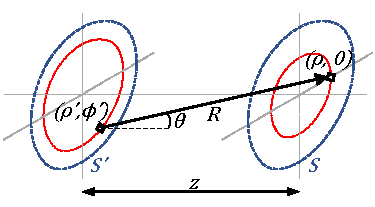
\includegraphics[width=10cm]{images/diffraction.pdf}
 \caption{Application of the Huygens-Fresnel principle to beam propagation from plane \(S'\) to plane \(S\) in a system with cylindrical symmetry.}
 \label{fig:diffraction}
\end{figure}
According to the Huygens-Fresnel principle, the field \(E\) at a point on plane \(S\) is defined as a superposition of secondary waves emitted from every point of plane \(S'\)~\cite{BornWolf-1999}. This can be expressed in the case of cylindrical symmetry as~\cite{Siegman-1986,PeatrossWare-2015}:
\begin{subequations} \label{eq:DI}
 \begin{align}
  &E(\rho) = -\frac{i}{\lambda} \int_{\rho'=0}^{\infty} E'(\rho') \int_{\phi'=0}^{2\pi} \frac{e^{ikR}}{R} K d\phi' \rho' d\rho' \label{eq:DI2a}\\
  &R = \sqrt{\rho^2 + \rho'^2 + z^2 - 2\rho\rho'\cos\phi'} \label{eq:DI2b}\\
  &K = \cos\theta = \frac{z}{R} \label{eq:DI2c}
 \end{align}
\end{subequations}
where \(\lambda\) is the wavelength, \(k = 2\pi / \lambda\) the wavenumber, and \(K\) the obliquity factor as it appears in Rayleigh-Sommerfeld diffraction theory.

Since the field on the output plane \(S\) does not depend on the angular coordinate \(\phi\), \(\phi = 0\) is chosen for the simplification of Eq.~\ref{eq:DI}.

Direct numerical integration of Eq.~\ref{eq:DI}, with \(O(N^3)\) complexity, is very time-consuming. Therefore, an approximation is usually employed to accelerate computations. The most well-known approximation is Fresnel diffraction, which assumes:
\begin{equation} \label{eq:FreA}
 \begin{split}
  &K \approx 1\\
  &R \approx
  \begin{cases}
   z & \text{(denominator)}\\
   z \left(1 + \frac{\rho^2 + \rho'^2 - 2\rho\rho'\cos\phi'}{2z^2}\right) & \text{(exponent)}
  \end{cases}
 \end{split}
\end{equation}
where "denominator" and "exponent" indicate the position of the \(R\) variable in Eq.~\ref{eq:DI2a}.

Substituting Eq.~\ref{eq:FreA} into Eq.~\ref{eq:DI2a} and using the formula
\begin{equation} \label{eq:formula}
 \int_{0}^{2\pi} e^{\pm i a \cos\phi}  d\phi = 2 \pi J_0(a)
\end{equation}
where \(J\) is the Bessel function, we obtain the expression for Fresnel diffraction with cylindrical symmetry:
\begin{equation} \label{eq:Fre}
 E(\rho) \approx -\frac{2 \pi i e^{ik\left(z+\frac{k\rho^2}{2z}\right)}}{\lambda z}
 \int_0^\infty E'(\rho') e^{i\frac{k\rho'^2}{2z}} J_0 \left(\frac{k\rho\rho'}{z}\right) \rho' d\rho'
\end{equation}

\textbf{\texttt{co2amp}} supports both Rayleigh-Sommerfeld (Eq.~\ref{eq:DI}) and Fresnel (Eq.~\ref{eq:Fre}) based propagation methods. Users can also choose to ignore the \texttt{pulse} evolution during free-space propagation.

Eqs.~\ref{eq:DI} and \ref{eq:Fre} assume monochromatic light, which is not the case for ultrashort pulses that possess a non-negligible bandwidth. Therefore, in \textbf{\texttt{co2amp}}, propagation is calculated in the frequency domain: Eqs.~\ref{eq:DI} or \ref{eq:Fre} are applied to the Fourier-transformed field at each node of the frequency calculation grid. Afterward, an inverse Fourier transform is used to return to the time domain.



%%%%%%%%%%%%%%%%%%%%%%%%%%%%%%%%%%%%%%%%%%%%%%%%%%%%%%%%%%%%%%%%%%%%%%%%%%%%%%%%%
\section{\texttt{Optic} Type A: \textit{Active Medium}}
The \textit{Active Medium} is the most complex type of \texttt{optic} that can be utilized in a \textbf{\texttt{co2amp}} project. Detailed models used for simulating molecular dynamics and \texttt{pulse} amplification are described in a dedicated Chapter~\ref{chapter:models}.

A configuration file for an \texttt{optic} of type A must include specifications of the gas mixture, pumping mechanism, and laser transitions considered in the simulations. An example of such a configuration file is provided below:

\begin{verbatim}
#=========================
# AM1.yml from 'examples/ATF 5 TW/ATF 3 final amplifier.co2' project

# Semi-diameter of the limiting aperture, m
semiDia: 45e-3

# Length of active medium, m
L: 0.57

# Gas mixture (bar)
p_CO2: 0.50
p_N2:  0.25
p_He:  7.50
O18:   0.472
C13:   0
T0:    300

# Bands included in calculations
band_reg: true
band_seq: true
band_hot: true

# Pumping
pumping: discharge
# Discharge volume, m^3
Vd: 0.0085
# Inter-electrode distance, m
D:  0.085
# Discharge profile
discharge: |
    0.00E+00 0.00000E+00 5.80000E+05
    1.00E-08 1.97186E+03 5.66356E+05
    2.00E-08 3.81445E+03 5.53030E+05
    3.00E-08 5.53410E+03 5.40019E+05
    4.00E-08 7.13691E+03 5.27312E+05
    ...
#=========================
\end{verbatim}

The composition of the active medium, including isotopic enrichment of carbon dioxide, and the initial temperature are specified under the "Gas mixture (bar)" section.

For discharge pumping, the geometry of the discharge and its temporal profile are required. In the case of optical pumping, the wavelength, absorption cross-section, and the temporal profile of the pumping pulse must be provided.

The 'optic~A~(discharge~pumped~CO2~amplifier).yml' and 'optic~A~(optically~pumped~CO2~amplifier).yml' template files contain detailed information on the configuration file format and can be referred to for further guidance.


%%%%%%%%%%%%%%%%%%%%%%%%%%%%%%%%%%%%%%%%%%%%%%%%%%%%%%%%%%%%%%%%%%%%%%%%%%%%%%%%%
\section{\texttt{Optic} Type P: \textit{Probe}}
A \textit{Probe} is a passive type of \texttt{optic}. It does not alter the field that fits within its semi-diameter. This can be expressed mathematically as:

\begin{equation}
E(t,\rho) = E'(t,\rho)
\end{equation}
where \( E'(t,\rho) \) and \( E(t,\rho) \) represent the field before and after passing through an \texttt{optic}, respectively.

However, a \textit{Probe} \texttt{optic} can serve as a limiting aperture, exhibiting zero transmittance for \( \rho > \text{semiDia} \). The sole configuration parameter for an \texttt{optic} of type P is its semi-diameter. An example of a configuration file for a \textit{Probe} with a 25 mm semi-diameter is shown below:

\begin{verbatim}
#=========================
# probe

semiDia: 25e-3
#=========================
\end{verbatim}


%%%%%%%%%%%%%%%%%%%%%%%%%%%%%%%%%%%%%%%%%%%%%%%%%%%%%%%%%%%%%%%%%%%%%%%%%%%%%%%%%
\section{\texttt{Optic} Type F: \textit{Spatial Filter}}
A \textit{Spatial Filter} applies a specified coordinate-dependent transmittance function to a \texttt{pulse}:

\begin{equation}
E(t,\rho) = E'(t,\rho) \sqrt{\mathcal{T}(\rho)}
\end{equation}
where \( \mathcal{T}(\rho) \) is the transmittance function, as defined in the configuration file.

An example configuration for a \textit{Spatial Filter} is shown below:

\begin{verbatim}
#=========================
# spatial filter

semiDia: 25e-3

filter: SIN
R: 10e-3
w: 10e-3
#=========================
\end{verbatim}

For more details and configuration options, refer to the 'optic~F~(spatial~filter).yml' template file.


%%%%%%%%%%%%%%%%%%%%%%%%%%%%%%%%%%%%%%%%%%%%%%%%%%%%%%%%%%%%%%%%%%%%%%%%%%%%%%%%%
\section{\texttt{Optic} Type S: \textit{Spectral Filter}}
A \textit{Spectral Filter} applies a specified frequency-dependent transmittance function to a \texttt{pulse}:

\begin{equation}
 \begin{aligned}
  &\widehat{E}'(\nu,\rho) = \mathcal{F}(E'(t,\rho))\\
  &\widehat{E}(\nu,\rho) = \widehat{E}'(\nu,\rho) \sqrt{\mathcal{T}(\nu)}\\
  &E(t,\rho) = \mathcal{F}^{-1}(\widehat{E}(\nu,\rho))
 \end{aligned}
\end{equation}
where \( \mathcal{F} \) and \( \mathcal{F}^{-1} \) denote the Fourier transform and the inverse Fourier transform, respectively, \( \nu \) is the frequency, and \( \mathcal{T}(\nu) \) is the transmittance function as defined in the configuration file.

An example configuration for a \textit{Spectral Filter} is provided below:

\begin{verbatim}
#=========================
# spectral filter

semiDia: 25e-3

filter: FREEFORM
form: |
    32.0e12 1.0
    32.1e12 0.9
    32.2e12 0.7
    32.3e12 0.5
    32.4e12 0.3
    32.5e12 0.0
    32.6e12 0.3
    32.7e12 0.5
    32.8e12 0.7
    32.9e12 0.9
    33.0e12 1.0
#=========================
\end{verbatim}

For further details and configuration options, refer to the 'optic~S~(spectral~filter).yml' template file.



%%%%%%%%%%%%%%%%%%%%%%%%%%%%%%%%%%%%%%%%%%%%%%%%%%%%%%%%%%%%%%%%%%%%%%%%%%%%%%%%%
\section{\texttt{Optic} Type L: \textit{Lens}}
A \textit{Lens} functions as a standard optical lens within the system:

\begin{equation}
 \begin{aligned}
  &\widehat{E}'(\nu,\rho) = \mathcal{F}(E'(t,\rho))\\
  &\widehat{E}(\nu,\rho) = \widehat{E}'(\nu,\rho) \exp\left( -\frac{i k \rho^2}{2 F} \right)\\
  &E(t,\rho) = \mathcal{F}^{-1}(\widehat{E}(\nu,\rho))
 \end{aligned}
\end{equation}
where \( k = \frac{2\pi\nu}{c} \) is the wave number (\( c \) is the speed of light) and \( F \) is the focal length of the lens.

The calculation is performed in the frequency domain to ensure that the effective focal length remains consistent across all frequencies in the pulse spectrum.

An example configuration for a lens with a 1-meter focal length is shown below:

\begin{verbatim}
#=========================
# lens (F = 1 m)

semiDia: 25e-3

F: 1.0
#=========================
\end{verbatim}


%%%%%%%%%%%%%%%%%%%%%%%%%%%%%%%%%%%%%%%%%%%%%%%%%%%%%%%%%%%%%%%%%%%%%%%%%%%%%%%%%
\section{\texttt{Optic} Type M: \textit{Material}}

In cases of oblique incidence, the effective intensity \(I_{\text{eff}}\) is reduced and the propagation distance in the material (effective thickness) \(\Theta_{\text{eff}}\) is automatically adjusted based on the incidence angle \(\theta_i\) and the refractive index \(n\):

\begin{equation}
 \begin{aligned}
   &\theta_r = \arcsin\left(\frac{\sin\theta_i}{n_0}\right)\\
   &I_{\text{eff}} = I \frac{\cos\theta_i}{\cos\theta_r}\\
   &\Theta_{\text{eff}} = \frac{\Theta}{\cos\theta_r} 
 \end{aligned}
\end{equation}
where \(I\) and \(\Theta\) are the intensity before the \texttt{optic} and the actual thickness of the material, respectively, and \(\theta_r\) is the refraction angle.

\subsubsection{Linear Dispersion and Absorption}
\begin{equation}
 \begin{aligned}
  &\widehat{E}'(\nu,\rho) = \mathcal{F}(E'(t,\rho))\\
  &\widehat{E}(\nu,\rho) = \widehat{E}'(\nu,\rho) \exp (2 \pi i \Delta \nu) \sqrt{\exp(-\alpha_0 \Theta_{\text{eff}})}\\
  &E(t,\rho) = \mathcal{F}^{-1}(\widehat{E}(\nu,\rho))
 \end{aligned}
\end{equation}
where \(\Delta \nu\) is defined as:
\begin{equation}\label{eq:Delta_nu_disp}
 \Delta \nu = \int_0^{\nu} (\nu'-\nu_c) \frac{dt}{d\nu'} d\nu',
\end{equation}
\begin{equation}
 \frac{dt}{d\nu'} = \frac{\Theta_{\text{eff}}}{c} \frac{dn_{g}}{d\nu'},
\end{equation}
with \(c\) as the speed of light, \(n_{g}\) as the group index of refraction, and \(\nu_c\) as the central frequency. The dispersion formulas used for calculating \(n_{g}\) are given in Appendix~\ref{appendix:optical_constants}.

\subsubsection{Nonlinear Interaction}
\begin{equation}
 \begin{aligned}
  &E(t,\rho) = E'(t,\rho) \exp\left(2\pi i \nu_c \frac{\Theta_{\text{eff}}}{c} n_2 I_{\text{eff}}(t,\rho)\right)\\
  &I_{\text{eff}}(t,\rho) = 2 h \nu_c (E'(t,\rho))^2 \frac{\cos\theta_i} {\cos\theta_r}
 \end{aligned}
\end{equation}
where \(n_2\) is the nonlinear refractive index, \(h\) is Planck's constant, and \(I(t,r)\) is the field intensity. Numerical values of \(n_2\) used in the program are given in Appendix~\ref{appendix:optical_constants}.

Configuration example for a \textit{Material} \texttt{optic}:

\begin{verbatim}
#=========================
# material

semiDia: 25e-3

material:  NaCl
thickness: 100e-3
tilt: 0
slices: 10
#=========================
\end{verbatim}

Currently supported materials include AgBr, AgCl, \ce{BaF2}, CdTe, CsI, GaAs, Ge, IRG22 (AMTIR1), IRG24, IRG25, KBr, KCl, KRS5, NaCl, NaF, Si, \ce{SiO2}, ZnS, ZnSe, and air. An arbitrary \(n_2\) can be specified in the configuration file, with a predefined value used otherwise (see Appendix~\ref{appendix:optical_constants}). To enhance accuracy, the \textit{Material} \texttt{optic} can be divided into several layers. A split-step method is employed for calculating linear and nonlinear interactions with a layer: first, a nonlinear interaction with a half-layer is calculated, followed by a full-layer linear interaction, and then a half-layer nonlinear interaction again.



%%%%%%%%%%%%%%%%%%%%%%%%%%%%%%%%%%%%%%%%%%%%%%%%%%%%%%%%%%%%%%%%%%%%%%%%%%%%%%%%%
\section{\texttt{Optic} Type C: \textit{Chirper}}
A \textit{Chirper} introduces a chirp to a pulse and is typically used to model a stretcher or compressor.

\begin{equation}
\begin{aligned}
&\widehat{E}'(\nu,\rho) = \mathcal{F}(E'(t,\rho))\\
&\widehat{E}(\nu,\rho) = \widehat{E}'(\nu,\rho) \exp(2 \pi i \Delta\nu)\\
&E(t,\rho) = \mathcal{F}^{-1}(\widehat{E}(\nu,\rho))
\end{aligned}
\end{equation}
where 
\begin{equation}\label{eq:Delta_nu_chirp}
 \Delta \nu = \int_0^{\nu} (\nu'-\nu_c) \frac{dt}{d\nu'} d\nu',
\end{equation}
\(\nu_c\) is the central frequency, and \(\frac{d\nu}{dt}\) is the chirpyness.

In the case of linear chirp, the chirpyness is constant, and Eq.~\ref{eq:Delta_nu_chirp} simplifies to:

\begin{equation}
\begin{aligned}
&\Delta \nu = \int_0^{\nu} \frac{\nu'-\nu_c}{\mathcal{C}} d\nu' = \frac{(\nu-\nu_c)^2}{2\mathcal{C}}\\
&\mathcal{C} = \frac{d\nu}{dt}
\end{aligned}
\end{equation}

An example configuration for a \textit{Chirper} with linear chirp is shown below:

\begin{verbatim}
#=========================
# stretcher (positive chirpyness => red chirp)

semiDia: 25e-3

chirp: LINEAR
c: 3.5e21
#=========================
\end{verbatim}

Currently, only linear chirp is supported in the program.

